%%
%% presentation.tex
%%
%% Made by Jakub Kuźma
%% Login   <kuba@jah.pl>
%%
%% Started on  Fri Oct 24 19:44:04 2008 Jakub Kuźma
%% Last update Fri Oct 24 19:44:04 2008 Jakub Kuźma
%%

\documentclass[12t]{beamer}
\usepackage[utf8]{inputenc}
\usepackage[T2A]{fontenc}
\usepackage[polish]{babel}
\usepackage{polski}
\usepackage{graphicx}
\usepackage{color}
%%
%% pygments.tex
%%
%% Made by Jakub Kuźma
%% Login   <kuba@ibm>
%%
%% Started on  Sat Oct 25 02:13:17 2008 Jakub Kuźma
%% Last update Sat Oct 25 02:13:17 2008 Jakub Kuźma
%%

\usepackage{fancyvrb}
\usepackage{color}

\newcommand\at{@}
\newcommand\lb{[}
\newcommand\rb{]}
\newcommand\PYbg[1]{\textcolor[rgb]{0.00,0.50,0.00}{\textbf{#1}}}
\newcommand\PYbf[1]{\textcolor[rgb]{0.73,0.40,0.53}{\textbf{#1}}}
\newcommand\PYbe[1]{\textcolor[rgb]{0.40,0.40,0.40}{#1}}
\newcommand\PYbd[1]{\textcolor[rgb]{0.73,0.13,0.13}{#1}}
\newcommand\PYbc[1]{\textcolor[rgb]{0.00,0.50,0.00}{\textbf{#1}}}
\newcommand\PYbb[1]{\textcolor[rgb]{0.40,0.40,0.40}{#1}}
\newcommand\PYba[1]{\textcolor[rgb]{0.00,0.00,0.50}{\textbf{#1}}}
\newcommand\PYaJ[1]{\textcolor[rgb]{0.73,0.13,0.13}{#1}}
\newcommand\PYaK[1]{\textcolor[rgb]{0.00,0.00,1.00}{#1}}
\newcommand\PYaH[1]{\fcolorbox[rgb]{1.00,0.00,0.00}{1,1,1}{#1}}
\newcommand\PYaI[1]{\textcolor[rgb]{0.69,0.00,0.25}{#1}}
\newcommand\PYaN[1]{\textcolor[rgb]{0.00,0.00,1.00}{\textbf{#1}}}
\newcommand\PYaO[1]{\textcolor[rgb]{0.00,0.00,0.50}{\textbf{#1}}}
\newcommand\PYaL[1]{\textcolor[rgb]{0.73,0.73,0.73}{#1}}
\newcommand\PYaM[1]{\textcolor[rgb]{0.74,0.48,0.00}{#1}}
\newcommand\PYaB[1]{\textcolor[rgb]{0.00,0.25,0.82}{#1}}
\newcommand\PYaC[1]{\textcolor[rgb]{0.67,0.13,1.00}{#1}}
\newcommand\PYaA[1]{\textcolor[rgb]{0.00,0.50,0.00}{#1}}
\newcommand\PYaF[1]{\textcolor[rgb]{1.00,0.00,0.00}{#1}}
\newcommand\PYaG[1]{\textcolor[rgb]{0.10,0.09,0.49}{#1}}
\newcommand\PYaD[1]{\textcolor[rgb]{0.25,0.50,0.50}{\textit{#1}}}
\newcommand\PYaE[1]{\textcolor[rgb]{0.63,0.00,0.00}{#1}}
\newcommand\PYaZ[1]{\textcolor[rgb]{0.00,0.50,0.00}{\textbf{#1}}}
\newcommand\PYaX[1]{\textcolor[rgb]{0.00,0.50,0.00}{#1}}
\newcommand\PYaY[1]{\textcolor[rgb]{0.73,0.13,0.13}{#1}}
\newcommand\PYaR[1]{\textcolor[rgb]{0.10,0.09,0.49}{#1}}
\newcommand\PYaS[1]{\textcolor[rgb]{0.25,0.50,0.50}{\textit{#1}}}
\newcommand\PYaP[1]{\textcolor[rgb]{0.49,0.56,0.16}{#1}}
\newcommand\PYaQ[1]{\textcolor[rgb]{0.40,0.40,0.40}{#1}}
\newcommand\PYaV[1]{\textcolor[rgb]{0.00,0.00,1.00}{\textbf{#1}}}
\newcommand\PYaW[1]{\textcolor[rgb]{0.73,0.13,0.13}{#1}}
\newcommand\PYaT[1]{\textcolor[rgb]{0.50,0.00,0.50}{\textbf{#1}}}
\newcommand\PYaU[1]{\textcolor[rgb]{0.82,0.25,0.23}{\textbf{#1}}}
\newcommand\PYaj[1]{\textcolor[rgb]{0.00,0.50,0.00}{#1}}
\newcommand\PYak[1]{\textcolor[rgb]{0.73,0.40,0.53}{#1}}
\newcommand\PYah[1]{\textcolor[rgb]{0.63,0.63,0.00}{#1}}
\newcommand\PYai[1]{\textcolor[rgb]{0.10,0.09,0.49}{#1}}
\newcommand\PYan[1]{\textcolor[rgb]{0.67,0.13,1.00}{\textbf{#1}}}
\newcommand\PYao[1]{\textcolor[rgb]{0.73,0.40,0.13}{\textbf{#1}}}
\newcommand\PYal[1]{\textcolor[rgb]{0.25,0.50,0.50}{\textit{#1}}}
\newcommand\PYam[1]{\textbf{#1}}
\newcommand\PYab[1]{\textit{#1}}
\newcommand\PYac[1]{\textcolor[rgb]{0.73,0.13,0.13}{#1}}
\newcommand\PYaa[1]{\textcolor[rgb]{0.50,0.50,0.50}{#1}}
\newcommand\PYaf[1]{\textcolor[rgb]{0.25,0.50,0.50}{\textit{#1}}}
\newcommand\PYag[1]{\textcolor[rgb]{0.40,0.40,0.40}{#1}}
\newcommand\PYad[1]{\textcolor[rgb]{0.73,0.13,0.13}{#1}}
\newcommand\PYae[1]{\textcolor[rgb]{0.40,0.40,0.40}{#1}}
\newcommand\PYaz[1]{\textcolor[rgb]{0.00,0.63,0.00}{#1}}
\newcommand\PYax[1]{\textcolor[rgb]{0.60,0.60,0.60}{\textbf{#1}}}
\newcommand\PYay[1]{\textcolor[rgb]{0.00,0.50,0.00}{\textbf{#1}}}
\newcommand\PYar[1]{\textcolor[rgb]{0.10,0.09,0.49}{#1}}
\newcommand\PYas[1]{\textcolor[rgb]{0.73,0.13,0.13}{\textit{#1}}}
\newcommand\PYap[1]{\textcolor[rgb]{0.00,0.50,0.00}{#1}}
\newcommand\PYaq[1]{\textcolor[rgb]{0.53,0.00,0.00}{#1}}
\newcommand\PYav[1]{\textcolor[rgb]{0.00,0.50,0.00}{\textbf{#1}}}
\newcommand\PYaw[1]{\textcolor[rgb]{0.40,0.40,0.40}{#1}}
\newcommand\PYat[1]{\textcolor[rgb]{0.10,0.09,0.49}{#1}}
\newcommand\PYau[1]{\textcolor[rgb]{0.40,0.40,0.40}{#1}}


\usetheme{Pittsburgh}

\author{Silesian Ruby Users' Group}
\title{Ruby on Rails}
\setbeamercovered{transparent}
%\setbeameroption{show notes}

\begin{document}

\frame{\titlepage}

\section{Wstęp}
\begin{frame}
  \frametitle{Dlaczego web development?}
  \begin{itemize}
  \item przenośność
  \item niezależność od systemów operacyjnych i przeglądarek
  \item łatwe zarządzanie i utrzymanie
  \end{itemize}
\end{frame}

\begin{frame}
  \frametitle{Dlaczego Ruby on Rails?}
  \begin{itemize}
  \item przyjemność z programowania
  \item open source
  \item czytelność kodu
  \item propagowanie dobrych praktyk programistycznych
  \item szybkość programowania
  \item łatwość reagowania na zmiany
  \item niezależność od systemu operacyjnego
  \item niezależność od środowiska pracy (NetBeans, RadRails, Emacs,
    Vim, JEdit)
  \end{itemize}
\end{frame}

\section{Ruby}
\begin{frame}
  \frametitle{Ruby}
  \begin{itemize}
  \item 1995 rok, Yukihiro Matsumoto aka Matz
  \item inspirowany przez CLU, Eiffel, Lisp, Perl, Python, Smalltalk
  \item interpretowany
  \item wieloparadygmatowy
  \item bardzo wysokiego poziomu (VHLL)
  \item w pełni obiektowy
  \end{itemize}
\end{frame}

\begin{frame}
  \frametitle{Cechy}
  \begin{itemize}
  \item dziedziczenie jednobazowe
  \item moduły - rodzaj dziedziczenia wielobazowego pozwalający
    włączyć gotową implementację zbioru metod do danej klasy
    (\emph{mixin})
    \note[item]{Moduły pełnią też rolę przestrzeni nazw}
  \item dziedziczenia używa się znacznie oszczędniej i rzadziej niż
    np. w Javie
  \end{itemize}
\end{frame}

\begin{frame}
  \frametitle{Cechy, c.d.}
  \begin{itemize}
  \item bogata biblioteka standardowa
  \item garbage collector
  \item przeciążanie operatorów
  \item liczby całkowite o dowolnych rozmiarach
  \item wyrażenia regularne wbudowane w składnię
  \end{itemize}
\end{frame}

\subsection{Ruby - implementacje}
\begin{frame}
  \frametitle{Ruby - implementacje}
  \begin{itemize}
  \item interpretery: MRI, Ruby Enterprise, JRuby, IronRuby
  \item maszyny wirtualne: MagLev, Rubinius, YARV
  \end{itemize}
\end{frame}

\begin{frame}[fragile]
  \frametitle{Samokomentujący się kod}
  \input{selfcomment1}
\end{frame}

\begin{frame}[fragile]
  \frametitle{Nazewnictwo}
  \begin{small}
    \input{naming1}
  \end{small}
  \note{Styl formatowania kodu nie jest narzucony z góry, wcięcia nie
    mają dla interpretera żadnego znaczenia}
\end{frame}

\begin{frame}[fragile]
  \frametitle{Stałe są zmienne}
  \input{consts1}
\end{frame}

\begin{frame}[fragile]
  \begin{itemize}
  \item omijane przez garbage collector
  \item wykorzystywane m.in. jako klucze w tablicach asocjacyjnych
  \end{itemize}
  \frametitle{Symbole}
  \begin{block}{Przykład}
    \input{symbols1}
  \end{block}
\end{frame}

\begin{frame}[fragile]
  \frametitle{Podstawowe elementy - tablice i hasze}
  \input{ruby1}
\end{frame}

\begin{frame}
  \begin{quote}
    “If it walks like a duck and quacks like a duck, I would call it a
    duck.”

    \hfill James Whitcomb Riley
  \end{quote}
\end{frame}

\begin{frame}
  \frametitle{Duck typing}
  \begin{itemize}
  \item rozpoznawanie typów na podstawie ich zachowania, a nie deklaracji
  \end{itemize}
\end{frame}

\begin{frame}
  \frametitle{Duck typing - przykład}
 \begin{footnotesize}
    \input{ducktyping1}
  \end{footnotesize}
\end{frame}

\begin{frame}
  \frametitle{Domknięcia}
  \begin{itemize}
  \item bloki kodu mogą być przekazywane jako argumenty i zwracane
    jako wynik działania funkcji (metody)
  \item są podstawową cechą języków funkcyjnych
  \item odwołują się do zmiennych z kontekstu, w którym zostały
    stworzone, a nie z którego są wywoływane
  \end{itemize}
\end{frame}

\begin{frame}
  \frametitle{Domknięcia - przykład}
  \input{closures1}
\end{frame}

\begin{frame}
  \frametitle{Domknięcia - wykorzystanie}
  \input{closures2}
\end{frame}

\subsection{Otwarte klasy}
\begin{frame}
  \frametitle{Otwarte klasy - przykład}
  \begin{Verbatim}[commandchars=@\[\]]
@PYay[class] @PYaN[Array]
  @PYay[def] @PYaK[shuffle]
    sort_by { @PYaX[rand] }
  @PYay[end]
  @PYay[def] @PYaK[shuffle!]
    @PYaX[self]@PYbe[.]replace shuffle
  @PYay[end]
@PYay[end]

a @PYbe[=] @PYbe[@lb[]]@PYag[1], @PYag[2], @PYag[3], @PYag[4], @PYag[5], @PYag[6], @PYag[7], @PYag[8], @PYag[9]@PYbe[@rb[]]
a@PYbe[.]shuffle!
@PYaf[#=> @lb[]2, 9, 4, 5, 1, 7, 8, 3, 6@rb[]]
\end{Verbatim}

  \note{Uzupełniamy klasę z biblioteki standardowej - używamy metody
    shuffle tak jakby była tam od zawsze.}
  \note{Ze względu na częste użycie metoda shuffle znalazła się w
    bibliotece standardowej w Ruby 1.8.7}
\end{frame}

\subsection{Monkey patching}
\begin{frame}
  \frametitle{Monkey patching - problem}
  \begin{Verbatim}[commandchars=@\[\]]
@PYay[class] @PYaN[Array]
  alias_method @PYat[:old_index], @PYat[:index]

  @PYay[def] @PYaK[index](obj @PYbe[=] @PYaj[nil])
    @PYay[if] obj@PYbe[.]nil?
      @PYaX[self]@PYbe[.]each_with_index @PYay[do] @PYbe[|]e, i@PYbe[|]
        @PYay[return] i @PYay[if] @PYay[yield] e
      @PYay[end]
      @PYaj[nil]
    @PYay[else]
      old_index(obj)
    @PYay[end]
  @PYay[end]
@PYay[end]
\end{Verbatim}

  \note{Fajnie byłoby, gdyby metoda index przyjmowała blok i zwróciła
    w tym przypadku index równy 6}
\end{frame}

\begin{frame}
  \frametitle{Monkey patching - rozwiązanie}
  \begin{Verbatim}[commandchars=@\[\]]
array @PYbe[=] @PYbe[@lb[]]@PYag[1], @PYag[7], @PYag[2], @PYag[8], @PYag[7], @PYag[10], @PYag[15], @PYag[2], @PYag[11]@PYbe[@rb[]]

array@PYbe[.]index { @PYbe[|]element@PYbe[|] element @PYbe[>] @PYag[10] }
@PYaf[#=> 6]
array@PYbe[.]index(@PYag[8])
@PYaf[#=> 3]
\end{Verbatim}

  \note{Podobnie jak w poprzednim przypadku - metoda index przyjmuje
    blok w Ruby 1.8.7}
\end{frame}

\subsection{Metaprogramowanie}
\begin{frame}
  \frametitle{Metaprogramowanie}
  \begin{itemize}
  \item metaprogramowanie w Rubim jest \textbf{proste}
  \item dysponujemy programowalnym językiem programowania
  \item główne narzędzie służące do budowy tzw. DSL
  \end{itemize}
\end{frame}

\begin{frame}[fragile]
  \frametitle{Metaprogramowanie - przykład}
  \begin{Verbatim}[commandchars=@\[\]]
@PYay[class] @PYaN[Module]
  @PYay[def] @PYaK[my_attr_accessor](@PYbe[*]symbols)
    symbols@PYbe[.]each @PYay[do] @PYbe[|]symbol@PYbe[|]
      @PYaX[module_eval] @PYap[%{]@PYap[def ]@PYbf[#{]symbol@PYbf[}]
@PYap[                      @at[]]@PYbf[#{]symbol@PYbf[}]
@PYap[                    end]@PYap[}]
      @PYaX[module_eval] @PYap[%{]@PYap[def ]@PYbf[#{]symbol@PYbf[}]@PYap[=(value)]
@PYap[                      @at[]]@PYbf[#{]symbol@PYbf[}]@PYap[ = value]
@PYap[                    end]@PYap[}]
    @PYay[end]
  @PYay[end]
@PYay[end]
\end{Verbatim}

\end{frame}

\begin{frame}[fragile]
  \frametitle{Metaprogramowanie - przykład, c.d.}
  \begin{Verbatim}[commandchars=@\[\]]
@PYay[class] @PYaN[Song]
  my_attr_accessor @PYat[:name], @PYat[:duration]
@PYay[end]

song @PYbe[=] @PYaq[Song]@PYbe[.]new
song@PYbe[.]name, song@PYbe[.]duration @PYbe[=] @PYaW["]@PYaW[Miles Davis - So What]@PYaW["], @PYag[565]
@PYaX[puts] @PYaW["]@PYbf[#{]song@PYbe[.]name@PYbf[}]@PYaW[, ]@PYbf[#{]song@PYbe[.]duration@PYbf[}]@PYaW[ s]@PYaW["]
\end{Verbatim}

  \note{To nie jest specjalna składnia - to zwykłe wywołanie metody
    zadeklarowanej w klasie Module}
\end{frame}

\begin{frame}[fragile]
  \frametitle{Metaprogramowanie - przykład, c.d.}
  \begin{Verbatim}[commandchars=@\[\]]
@PYay[class] @PYaN[Song]
  @PYay[def] @PYaK[name]
    @PYaR[@at[]name]
  @PYay[end]
  @PYay[def] @PYaK[name]@PYbe[=](value)
    @PYaR[@at[]name] @PYbe[=] value
  @PYay[end]
  @PYay[def] @PYaK[duration]
    @PYaR[@at[]duration]
  @PYay[end]
  @PYay[def] @PYaK[duration]@PYbe[=](value)
    @PYaR[@at[]duration] @PYbe[=] value
  @PYay[end]
@PYay[end]
\end{Verbatim}

  \note{Wiele osób w dalszym ciągu traci czas na pisanie getterów i
    setterów w np. Javie}
  \note{nie musimy pisać funkcji - attr_accessor, attr_reader,
    attr_writer są w bibliotece standardowej. Zostały napisane w C}
\end{frame}

\subsection{Użycie method\_missing}
\begin{frame}[fragile]
  \frametitle{Użycie method\_missing}
  \begin{Verbatim}[commandchars=@\[\]]
@PYay[class] @PYaN[Greetings]
  @PYay[def] @PYaK[method_missing](method_name, @PYbe[*]args)
    @PYay[if] method_name@PYbe[.]to_s @PYbe[=~] @PYak[/]@PYak[^say_hello_to_(.+)]@PYak[/]
      @PYaX[name] @PYbe[=] @PYar[$1]@PYbe[.]capitalize
      @PYaX[puts] @PYaW["]@PYaW[Hello, ]@PYbf[#{]@PYaX[name]@PYbf[}]@PYaW[!]@PYaW["]
    @PYay[else]
      @PYay[raise] @PYaq[NoMethodError],
        @PYaW["]@PYaW[undefined method `]@PYbf[#{]method_name@PYbf[}]@PYaW[' for ]@PYbf[#{]@PYaX[self]@PYbf[}]@PYaW["]
    @PYay[end]
  @PYay[end]
@PYay[end]
\end{Verbatim}

\end{frame}

\begin{frame}[fragile]
  \frametitle{Użycie method\_missing, c.d.}
  \begin{Verbatim}[commandchars=@\[\]]
greetings @PYbe[=] @PYaq[Greetings]@PYbe[.]new

greetings@PYbe[.]say_hello_to_world
@PYaf[# Hello, World!]

greetings@PYbe[.]say_goodbye_to_world
@PYaf[# NoMethodError: undefined method ...]
\end{Verbatim}

  \note{Dla zaoszczędzenia czasu nie będziemy prezentować jak osiągnąć
    ten efekt w tradycyjny sposób}
\end{frame}

\begin{frame}
  \frametitle{Podsumowanie}
  \begin{itemize}
  \item „pseudo-code that runs” - skupianie się na rozwiązaniu
    problemu, nie na języku
  \item język zaprojektowany \textbf{dla ludzi}
  \item radość z programowania
  \item TIMTOWTDI - wolność wyboru (jak w Perlu, przeciwnie niż w
    Pythonie)
  \item zasada najmniejszego zaskoczenia - Ruby jest intuicyjny
  \end{itemize}
  \note{Stworzony by cieszyć}
\end{frame}

\section{Ruby - dodatki}
\begin{frame}[fragile]
  \frametitle{Rake - Ruby Make}
  \begin{footnotesize}
    \input{rakefile1}
  \end{footnotesize}
\end{frame}

\begin{frame}[fragile]
  \frametitle{RSpec - framework BDD}
  \begin{footnotesize}
    \input{rspec1}
  \end{footnotesize}
\end{frame}

\begin{frame}[fragile]
  \frametitle{RubyGems}
  \begin{itemize}
  \item system paczek RubyGems
  \item zależności pomiędzy gemami
  \item łatwa aktualizacja gemów
  \item prawie 4000 gemów w repozytorium
  \end{itemize}
  \begin{block}{Przykład}
\begin{verbatim}
$ gem install rails
\end{verbatim}
  \end{block}
\end{frame}

\begin{frame}
  \begin{quote}
    “I always thought Smalltalk would beat Java. I just
    didn't know it would be called 'Ruby' when it did.”

    \hfill Kent Beck
  \end{quote}
\end{frame}

\section{Ruby on Rails}
\begin{frame}
  \frametitle{Ruby on Rails}
  \begin{itemize}
  \item David Heinemeier Hansson, 2004 r.
  \item kompletny framework do tworzenia aplikacji internetowych
    opartych o bazy danych
  \item wzorzec MVC
  \end{itemize}
\end{frame}

\begin{frame}
  \frametitle{Rails way}
  \begin{itemize}
  \item Convention over Configuration
  \item Don't Repeat Yourself
  \end{itemize}
\end{frame}

\begin{frame}
  \frametitle{Z czego składa się Rails?}
  \begin{itemize}
  \item ActiveRecord
  \item ActionPack
  \item ActiveResource
  \item ActionMailer
  \item ActiveSupport
  \end{itemize}
\end{frame}

\begin{frame}
  \frametitle{Architektura Rails}
  \begin{figure}
    \centering
    \includegraphics[width=\linewidth]{railsarchitecture.png}
  \end{figure}
\end{frame}

\begin{frame}[fragile]
  \frametitle{Zaczynamy!}
  \begin{columns}[T]
    \begin{column}{2.3cm}
      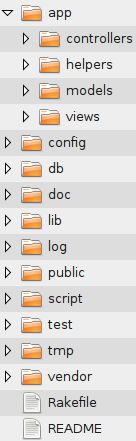
\includegraphics[width=2.3cm]{structure.png}
    \end{column}
    \begin{column}{7.5cm}
\begin{verbatim}
# gem install rails

$ rails myapp

$ cd myapp

$ ./script/server
\end{verbatim}
    \end{column}
  \end{columns}
\end{frame}

\begin{frame}
  \frametitle{ActiveRecord}
  \begin{itemize}
  \item domyślny ORM dla Rails
  \item są też inne opcje (np. DataMapper)
  \item implementacja wzorca Active Record
  \end{itemize}
\end{frame}

\begin{frame}
  \frametitle{ActiveRecord - co dostajemy?}
  \begin{itemize}
  \item prosta konfiguracja
  \item migracje bazy danych
  \item proste tworzenie asocjacji
  \item zapytania
  \item walidatory
  \item wywołania zwrotne
  \item transakcje
  \item kilka innych rzeczy
  \end{itemize}
\end{frame}

\begin{frame}[fragile]
  \frametitle{ActiveRecord - szybki start}
\begin{verbatim}
development:
  adapter: mysql
  database: demo
  username: admin
  password: password
  host: localhost
\end{verbatim}
\begin{verbatim}
$ ./script/generate model post title:string content:text

$ rake db:migrate
\end{verbatim}
  \input{configuration1}
\end{frame}

\begin{frame}
  \frametitle{ActiveRecord - migracje}
  \begin{itemize}
  \item proste w użyciu wersjonowanie schematu bazy, historia zmian
  \item Ruby zamiast SQL-a
    \note{Uzyskujemy przenośność pomiędzy różnymi silnikami
      bazodanowymi}
  \item praca w zespołach
  \end{itemize}
\end{frame}

\begin{frame}[fragile]
  \frametitle{ActiveRecord - migracje - przykład}
  \input{migrations1}
\end{frame}

\begin{frame}
  \frametitle{ActiveRecord - asocjacje}
  \begin{itemize}
  \item mapowanie powiązań pomiędzy obiektami ActiveRecord
  \item wyrażają relację takie jak “user has many projects” czy
    “product belongs to category”
  \item oparte na metaprogramowaniu
  \end{itemize}
\end{frame}

\begin{frame}[fragile]
  \frametitle{ActiveRecord - asocjacje - przykład}
  \input{associations1}
\end{frame}

\begin{frame}[fragile]
  \frametitle{ActiveRecord - asocjacje - przykład, c.d.}
  \input{associations2}
\end{frame}

\begin{frame}
  \frametitle{ActiveRecord - zapytania}
  \begin{itemize}
  \item Różne sposoby budowania zapytań
  \item Nazwane zapytania
  \end{itemize}
\end{frame}

\begin{frame}[fragile]
  \frametitle{ActiveRecord - przykłady zapytań}
  \begin{footnotesize}
    \input{finders1}
  \end{footnotesize}
\end{frame}

\begin{frame}[fragile]
  \frametitle{ActiveRecord - przykłady zapytań c.d.}
  \begin{footnotesize}
    \input{finders2}
  \end{footnotesize}
\end{frame}

\begin{frame}[fragile]
  \frametitle{ActiveRecord - przykłady zapytań c.d.}
  \begin{small}
    \input{finders3}
  \end{small}
\end{frame}

\begin{frame}
  \frametitle{Named scope - przykłady}
  \begin{small}
    \input{namedscope1}
  \end{small}
\end{frame}

\begin{frame}
  \frametitle{ActiveRecord - walidatory}
  \begin{itemize}
  \item gwarantują poprawność wprowadzanych danych
  \item przeniesienie walidacji z poziomu bazy danych do modelu
  \item można walidować: format, długość, obecność, unikalność,
    powiązane obiekty, etc.
  \item łatwe tworzenie własnych walidatorów
  \end{itemize}
\end{frame}

\begin{frame}
  \frametitle{ActiveRecord - walidatory - przykład}
  \input{validators1}
\end{frame}

\begin{frame}
  \frametitle{ActiveRecord - wywołania zwrotne}
  \begin{itemize}
  \item wyzwalanie logiki przed lub po zmianie stanu obiektu
  \item manipulacja atrybutami obiektu przed jego utworzeniem,
    zapisem, usunięciem lub walidacją
  \item przeniesienie logiki z kontrolera do modelu
  \end{itemize}
\end{frame}

\begin{frame}
  \frametitle{ActiveRecord - callbacks - przykład}
  \input{callbacks1}
\end{frame}

\begin{frame}
  \frametitle{ActiveRecord - transakcje}
  \begin{itemize}
  \item bloki kodu, w których gwarantowana jest atomowość wszystkich
    operacji na bazie danych
  \item różne modele w jednej transakcji
  \end{itemize}
  \begin{block}{Przykład}
    \input{transactions1}
  \end{block}
\end{frame}

\begin{frame}
  \frametitle{ActiveRecord}
  \begin{itemize}
  \item Single Table Inheritance
  \item asocjacje polimorficzne
  \item optimistic locking
  \item acts\_as: state\_machine, taggable, nested\_set, commentable,
    dictionary, geocodable
  \end{itemize}
\end{frame}

\begin{frame}
  \begin{quote}
    “I have never seen an Active Record implementation as complete or as useful as Rails”

    \begin{small}
      \hfill Martin Fowler, software architect
    \end{small}
  \end{quote}
  \note{M.Fowler jest autorem książek i znanym wykładowcą z tematyki
    architektury oprogramowania, specjalizującym się w analizie
    obiektowej i projektowaniu, UML, wzorcach projektowych, metodykach
    zwinnych, w tym Programowania ekstremalnego}
\end{frame}

\begin{frame}
  \frametitle{ActionPack}
  \begin{itemize}
  \item podział odpowiedzi aplikacji na dwie części:
    \begin{itemize}
    \item ActionController
    \item ActionView
    \end{itemize}
  \end{itemize}
\end{frame}

\begin{frame}
  \frametitle{ActionPack::ActionController}
  \begin{itemize}
  \item request zostaje skierowany do odpowiedniej akcji (routing)
  \item akcja zwraca odpowiedź do przeglądarki
    \begin{itemize}
    \item wyrenderowany widok
    \item przekierowanie
    \item błąd
    \end{itemize}
  \item cookies
  \item sesje
  \item flash
  \item filtry
  \end{itemize}
\end{frame}

\begin{frame}
  \frametitle{ActionController::Routing}
  \begin{itemize}
  \item wiązanie URI z akcjami odpowiednich kontrolerów
  \end{itemize}
  \begin{block}{Przykład}
    \input{routing1}
  \end{block}
\end{frame}

\begin{frame}
  \frametitle{ActionPack::ActionController}
  \begin{small}
  \input{actioncontroller1}
  \end{small}
\end{frame}

\begin{frame}
  \frametitle{ActionPack::ActionView}
  \begin{itemize}
  \item szablony w widokach: ERb, Haml, Liquid i inne
  \item partiale
  \item helpery
  \end{itemize}
\end{frame}

\begin{frame}[fragile]
  \frametitle{ActionPack::ActionView - index.html.erb}
  \input{erb1}
\end{frame}

\begin{frame}[fragile]
  \frametitle{ActionPack::ActionView - index.html.haml}
  \begin{footnotesize}
  \begin{columns}[T]
    \begin{column}{4cm}
      \begin{verbatim}
%table#beers.important
  %tr.header
    %th Name
    %th Type
  - @beers.each do |beer|
    %tr
      %td= beer.name
      %td= beer.type
\end{verbatim}

    \end{column}
    \begin{column}{6cm}
      \input{haml2}
    \end{column}
  \end{columns}
  \end{footnotesize}
\end{frame}

\begin{frame}
  \frametitle{ActiveSupport}
  \begin{Verbatim}[commandchars=@\[\]]
@PYaX[puts] @PYag[40]@PYbe[.]minutes@PYbe[.]ago @PYaf[#=> 2008-10-27 20:29:37 +0100]
@PYaX[puts] @PYag[20]@PYbe[.]weeks@PYbe[.]from_now @PYaf[#=> 2009-03-16 21:10:45 +0100]
@PYaX[puts] @PYaq[Time]@PYbe[.]now@PYbe[.]at_beginning_of_year
	@PYaf[#=> Tue Jan 01 00:00:00 +0100 2008]
\end{Verbatim}

\end{frame}

\begin{frame}
  \frametitle{Serwery HTTP}
  \begin{itemize}
  \item Webrick
  \item Mongrel, Thin, Ebb
  \item Passenger (Apache 2)
  \end{itemize}
\end{frame}

\begin{frame}
  \frametitle{Przykłady wdrożeń}
  \begin{itemize}
  \item Twitter
  \item Yellowpages
  \item Basecamp
  \item GitHub
  \item Shopify
  \item Slideshare
  \end{itemize}
\end{frame}

\section{Podsumowanie}
\begin{frame}
  \frametitle{Jak zacząć?}
  \begin{itemize}
  \item instant-rails
  \item github.com
  \item opensourcerails.com
  \item heroku.com
  \end{itemize}
\end{frame}

\begin{frame}
  \begin{quote}
    “Rails is the most well thought-out web development framework I've
    ever used. (...) Nobody has done it like this before.”

    \begin{small}
      \hfill James Duncan Davidson, Creator of Tomcat and Ant
    \end{small}
  \end{quote}
\end{frame}

\begin{frame}
  \begin{center}
    \begin{Large}
      Dziękujemy za wytrwałość!
    \end{Large}
  \end{center}
\end{frame}

\end{document}
